\documentclass{article}

\usepackage[left=1in, right=1in, top=1in, bottom=1in]{geometry}

\usepackage{setspace}
\usepackage{fancyhdr}
\usepackage{hyperref}
\usepackage{amsthm}
\usepackage{amssymb}
\usepackage{multirow}
\usepackage{enumitem}
\usepackage{graphicx}
\usepackage{makecell}
\usepackage{booktabs}
\usepackage{titlesec}
\usepackage{amsmath}
\usepackage{pdfpages}
\usepackage{enumitem}
\usepackage{caption}

\setcounter{secnumdepth}{4}

\hypersetup{
    colorlinks=true,     
    urlcolor=magenta
}

\renewcommand{\qedsymbol}{\rule{0.7em}{0.7em}}

\newlength\tindent
\setlength{\tindent}{\parindent}
\setlength{\parindent}{0pt}
\renewcommand{\indent}{\hspace*{\tindent}}
\setlength{\parskip}{0em}

\newenvironment{blockquote}{%
  \par%
  \vskip1em
  \leftskip=2em\rightskip=2em%
  \noindent\ignorespaces}{%
  \par\vskip1em}

\newenvironment{blockquote2}{%
	\par%
	\vskip1em
	\leftskip=4em\rightskip=4em%
	\noindent\ignorespaces}{%
	\par\vskip1em}

\pagestyle{fancy}
\fancyhf{}
\fancyhead[LO]{STA5176}
\fancyhead[RO]{Kyle Ligon}
\fancyfoot[LO]{Chapter 14 and 15}
\fancyfoot[RO]{\thepage}
 
\renewcommand{\headrulewidth}{0.5pt}
\renewcommand{\footrulewidth}{0.5pt}

\begin{document}
\section*{Chapter 14 and 15 Homework}
\subsection*{Due 4-8-2018}
\subsubsection*{Problem 14.8}
\subsubsection*{ (a) Assess ANOVA assumptions using the graph from PROC MIXED.}
The most concerning plot is the scatterplot with an apparent pattern as you increase the Group Mean.  Though, with a wonky residual histogram and Q-Q Plot that is overpredicting at the extremes this data does not appear to fit a trustworthy ANOVA scenario.  
\begin{figure}[h]
\centering
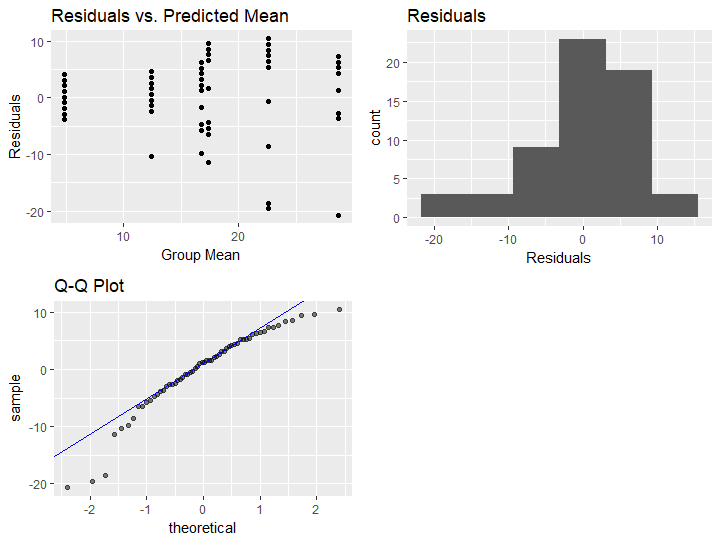
\includegraphics[width = 1.0\textwidth]{ANOVAcheck148.png}
\end{figure}
\pagebreak
\subsubsection*{(b) Perform an ANOVA to determine if there is an interaction between the age group and types of products; $\alpha$ = 0:05}
\begin{table}[ht]
\caption{ANOVA Table for Attention Spans}
\centering
\begin{tabular}{l c c c c c}
\hline\hline
Row Names & SS & df & MS & F & P-Value \\ [0.5ex] 
\hline
Main Effect \\ 
\hspace{3mm}Age Group & 1349.6333 & 2 & 674.81665 & 12.868 & 2.67x$10^{-5}$ \\
\hspace{3mm}Products & 1995.2667 & 1 & 1995.2667 & 38.048 & 9.15x$10^{-8}$\\
Interaction \\
\hspace{3mm}(Age Group:Products) & 14.2333 & 2 & 7.1167 & 0.136 & 0.873 \\
Error & 2831.8000 & 54 & 52.4407 \\
Total & 6190.9 & 59 &  \\ [1ex]
\hline
\end{tabular}
\label{table:nonlin}
\end{table}

Check the Interaction, Reject if $F_{Interaction} > F_{\alpha, df_{Interaction}, df_{Error}}$:
\begin{blockquote}
$F_{Interaction} = 0.873 < 3.1682 = F_{0.05, 2, 54}$ \\
Thus, the interaction is not significant and can be removed from the model.  
\end{blockquote}

\subsubsection*{(c) If there is an interaction, create a probability plot for age group and product type and provide an interpretation for the interaction}


Dealing with the Interaction Term
\begin{blockquote}
Since the Interaction term of AgeGroup:Products is not significant ($> F_{0.05, 2, 54} = 3.1682$), we will remove it from our ANOVA model and just look at the Main Effects.
\end{blockquote}


\subsubsection*{(d) If there is not an interaction, remove the interaction term, recompute the ANOVA table, and determine if there are main effects of age group and product type; $\alpha$ = 0:05}

\begin{table}[ht]
\caption{ANOVA Table for Attention Spans without Interaction Term}
\centering
\begin{tabular}{l c c c c c}
\hline\hline
Row Names & SS & df & MS & F & P-Value \\ [0.5ex] 
\hline
Main Effect \\ 
\hspace{3mm}Age Group & 1350 & 2 & 674.8 & 13.28 & 1.91x$10^{-5}$ \\
\hspace{3mm}Products & 1995 & 1 & 1995.3 & 39.26 & 5.60x$10^{-8}$\\
Error & 2846 & 56 & 50.8 \\
Total & 6191 & 59 &  \\ [1ex]
\hline
\end{tabular}
\label{table:nonlin}
\end{table}

Checking to see if the F Statistics Are Greater Than $F_{\alpha, df_{Main Effect}, df_{Error}}$
\begin{eqnarray}
F_{Age Group} = 13.28 > 3.1619 = F_{\alpha, df_{Main Effect}, df_{Error}}  \nonumber \\
F_{Products} = 13.28 > 4.0130 = F_{\alpha, df_{Main Effect}, df_{Error}}  \nonumber 
\end{eqnarray}

\begin{blockquote}
Both the Main Effects are statistically significant therefore, we should move onto Post Hoc testing to look at statistically different pairs.  
\end{blockquote}


\pagebreak
\subsubsection*{(e) Report significantly different pairs using Tukey's W and $\alpha$ = 0:05; REMEMBER: if there is an interaction present, we must account for that when performing post-hoc testing} 

\begin{blockquote}
To find which groups are different from each other, we will utilize Tukey's W to check which means are different from one another.  We will verify this by checking which  one's p-values are less than 0.05 after using the TukeyHSD test on our ANOVA model in R.  
\end{blockquote}

Conclusion/Interpretation:
\begin{blockquote}
With out Tukey W test being run, the differences lie in the following means:
\end{blockquote}
\begin{itemize}[leftmargin=+0.5in]
	\item[$\bullet$] $a_{2}$ and $a_{3}$ differs from $a_{1}$
	\item[$\bullet$] $p_{2}$ differs from $p_{1}$
\end{itemize}

\subsection*{15.10}

\subsubsection*{(a) Assess ANOVA assumptions using the graph from PROC MIXED.}
\begin{blockquote}
With a Residual scatter plot that does not have a readily apparent pattern, a Residual histogram that is mound shaped, and a Q-Q plot that fits the theoretical Normal model reasonably well, I feel confident using ANOVA on this data.   
\end{blockquote}
\begin{figure}[h]
\centering
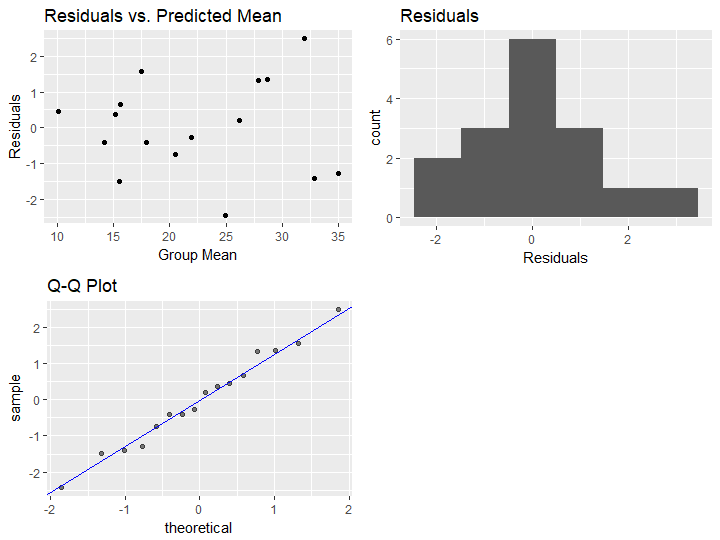
\includegraphics[width = 1.0\textwidth]{1510_block.png}
\end{figure}

\subsubsection*{(b) Determine if there is a difference between gasoline blends using ANOVA for Latin Square; $\alpha$ = 0:05}
\begin{table}[ht]
\caption{ANOVA Table for LSD Gasoline Brands}
\centering
\begin{tabular}{l c c c c c}
\hline\hline
Row Names & SS & df & MS & F & P-Value \\ [0.5ex] 
\hline 
Treatment/Gasoline Brand & 106.3 & 3 & 35.42 & 8.218 & 0.0151 \\
Row/Car Model & 8.3 & 3 & 2.78 & 0.644 & 0.6143 \\
Column/Driver & 755.4 & 3 & 251.79 & 58.412 & 7.84x$10^{-5}$ \\ 
Error & 25.9 & 6 & 4.31 \\
Total & 895.9 & 15 &  \\ [1ex]
\hline
\end{tabular}
\label{table:nonlin}
\end{table}

Hypotheses: 
\begin{blockquote}
$H_{0}: \mu_{A} = \mu_{B} = \mu_{C} = \mu_{D}$ \\
$H_{1}:$ at least one mean is different.   
\end{blockquote}

Test Statistic:
\begin{blockquote}
F = 8.218
\end{blockquote}

Rejection Region:
\begin{blockquote}
Reject if $F_{0} \geq F_{\alpha, df_{trt}, df_{error}}; F_{\alpha, df_{trt}, df_{error}} = 4.7571$
\end{blockquote}

Conclusion/Interpretation:
\begin{blockquote}
Since 8.218 $\geq$ 4.7571, we have strong enough evidence to reject the hypothesis that the means are the same.  There is evidence to suggest at least on mean is different from the others.  
\end{blockquote}

\subsubsection*{(c) If there is a difference per part (b), use Tukey's W to determine the significantly different pairs; $\alpha$ = 0:05}

\begin{blockquote}
To find which groups are different from each other, we will utilize Tukey's W to check which means are different from one another.  We will verify this by checking which  one's p-values are less than 0.05 after using the TukeyHSD test on our ANOVA model in R.
\end{blockquote}

Conclusion/Interpretation:
\begin{blockquote}
With out Tukey W test being run, the differences lie in the following means:
\end{blockquote}
\begin{itemize}[leftmargin=+0.5in]
	\item[$\bullet$] Brand B is bigger than Brand C.
	\item[$\bullet$] Brand D is larger than Brand C.
\end{itemize}

\subsubsection*{(d) From part (c), which blend (or blends) gives the highest gas mileage?}
No hierarchy jumps out based on Tukey W's analysis.  We can't tell which brand is on top.  All we can be "sure of" ($\alpha = 0.05$) is that Brand B and Brand D are bigger than Brand C.

\pagebreak
\subsubsection*{(e) Determine if there is a difference between gasoline blends using ANOVA for completely randomized designs (i.e., ignore the blocking factors); $\alpha$ = 0:05}
\begin{blockquote}
With the following ANOVA graphs, I am hesitant to put faith in any results from the ANOVA statistical test.  
\end{blockquote}

\begin{figure}[h]
\centering
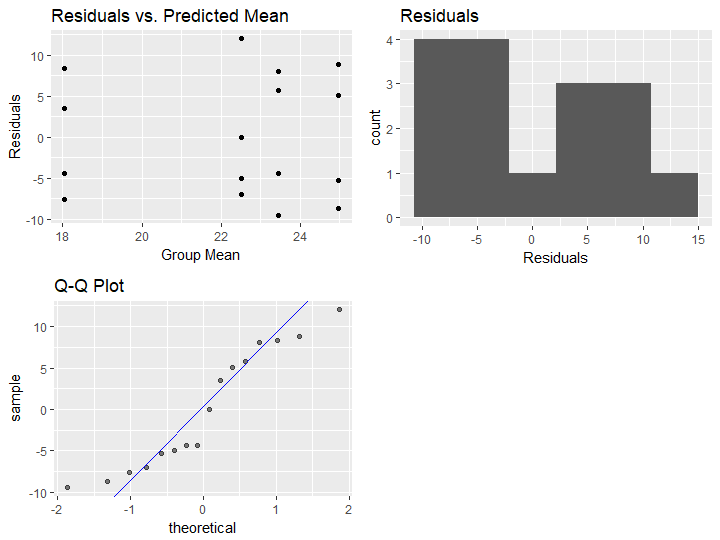
\includegraphics[width = 1.0\textwidth]{1510_noBlock.png}
\end{figure}

\begin{table}[ht]
\caption{ANOVA Table for Gasoline Brands ignoring Blocking Factors}
\centering
\begin{tabular}{l c c c c c}
\hline\hline
Row Names & SS & df & MS & F & P-Value \\ [0.5ex] 
\hline 
Treatment/Gasoline Brand & 106.3 & 3 & 35.4239 & 0.538 & 0.665 \\
Error & 789.6 & 12 & 65.80 \\
Total & 895.9 & 15 &  \\ [1ex]
\hline
\end{tabular}
\label{table:nonlin}
\end{table}

\pagebreak
Hypotheses:
\begin{blockquote}
$H_{0}: \mu_{A} = \mu_{B} = \mu_{C} = \mu_{D}$ \\
$H_{1}:$ at least one mean is different than the rest
\end{blockquote}

Test Statistic:
\begin{blockquote}
F = 0.538
\end{blockquote}

Rejection Region:
\begin{blockquote}
Reject $F_{0}$ if $F_{0} \geq F_{\alpha, df_{trt}, df_{error}}$.
$F_{\alpha, df_{trt}, df_{error}} = 3.4903$
\end{blockquote}

Conclusion/Interpretation:
\begin{blockquote}
Since our test statistic is less than the Rejection bound, we fail to reject the null hypothesis that the means are the same.  We do not have strong enough evidence to suggest that there is a mean different from the rest.  
\end{blockquote}

\subsubsection*{(e) Compare the MSE from part (b) to the MSE from part (e) - what happens when we ignore the blocking factors?}
\begin{blockquote}
The $MSE_{Brand}$ for the LSD was 35.42.  The $MSE_{Brand}$ for the ANOVA not blocked on Car Model and Driver was 35.4239.  Although their MSE are very similar, their difference lies in their $df_{error}$.  Since we split on Car Model and Driver in the first group, it allows for less error to be absorbed by the error term.     
\end{blockquote}

\subsubsection*{(f) Which would you say is the appropriate analysis?}
\begin{blockquote}
You could base this answer based solely on the PROC MIXED graphs for each group.  The winner would be the ANOVA including the blocking factors.  When we don't account for the blocking factors, the PROC MIXED graphs hardly represent a normal situation lending its resultant analysis null and void.  
\end{blockquote}


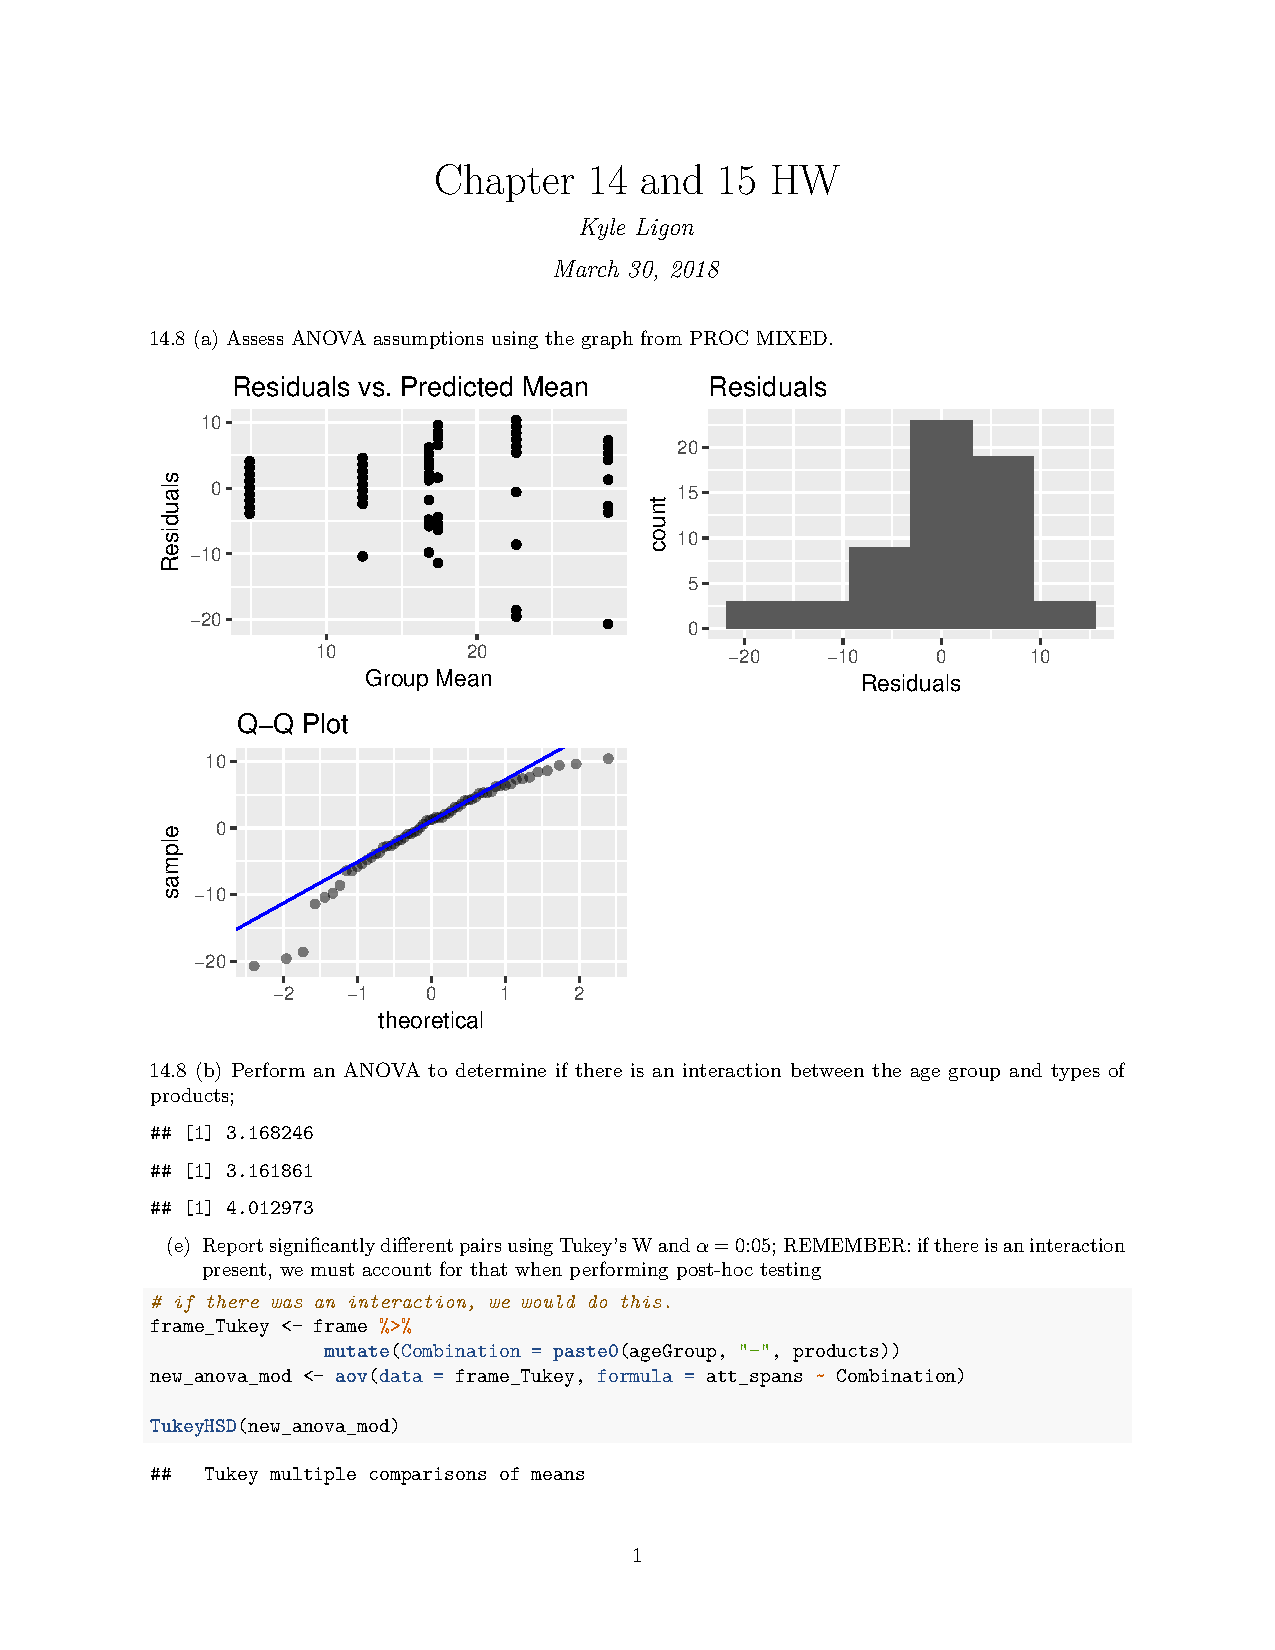
\includepdf[pages=-]{Chapter14_and_15_HW.pdf}

\end{document}















